\documentclass{beamer}

\usepackage{tikz}
\usetikzlibrary{positioning,matrix, arrows.meta}
\usetikzlibrary{graphdrawing.trees}
\usetikzlibrary{external}
\tikzexternalize % activate!
\usepackage{color}
\newcommand{\vet}[1]{\foreach \num in {#1}{\el{\num}}}
\newcommand{\vetempty}[1]{\foreach \num in {#1}{\elempty{\num}}}
\newcommand{\el}[1]{\tikz{\node[font=\smaller, draw]{#1}}}
\newcommand{\elempty}[1]{\tikz{\node[font=\small, minimum size=1cm, draw=white, fill=white]{#1}}}
\newcommand{\bl}{\color{blue}}
\newcommand{\gr}{\color{gray}}
\newcommand{\re}{\color{red}}
\newcommand{\tcb}[1]{\textcolor{blue}{#1}}
\newcommand{\tcg}[1]{\textcolor{green}{#1}}
\newcommand{\tcr}[1]{\textcolor{red}{#1}}
\newcommand{\ar}{\tikz{\draw [->] (0,0) -- (0,0.4)}}
\newcommand{\nd}{\color{white!0}.}

\usepackage{beamerthemeSingapore}
\usepackage{graphicx}
%\usepackage{here}
\usepackage{url}
\usepackage[brazil]{babel}
\usepackage[T1]{fontenc}
\usepackage[utf8]{inputenc}
%\usepackage[tight,raggedright]{subfigure}
\usepackage{subfigure}
\usepackage[alf]{abntex2cite}
\usepackage{listings}
\usepackage{minted}
\usepackage[linesnumbered,ruled,vlined]{algorithm2e}
\usepackage{amsmath}
\usepackage{pdfpages}
% Please add the following required packages to your document preamble:
\usepackage{booktabs}
\usepackage{ragged2e}
\usepackage{etoolbox}
\usepackage{mathtools}
\usepackage{caption}
\usepackage{xmpmulti}
\usepackage[usestackEOL]{stackengine}
\edef\tmp{\the\baselineskip}
\setstackgap{L}{\tmp}

\DeclareTextFontCommand{\textbf}{\bfseries}
\DeclareTextFontCommand{\textit}{\itshape}

\tikzset{
  treenode/.style = {align=center, inner sep=0pt, text centered,
    font=\sffamily},
  arn_bf/.style = {treenode, rectangle, rounded corners=.8ex, black, font=\sffamily\bfseries, draw=black,fill=white, text width=3.5em, inner sep=2pt },% arbre rouge noir, noeud noir
  arn_rf/.style = {treenode, rectangle, rounded corners=.8ex, red, font=\sffamily\bfseries, draw=red,fill=white, text width=3.5em, inner sep=2pt },% arbre rouge noir, noeud noir
  arn_bt/.style = {treenode, rectangle, rounded corners=.8ex, black, font=\sffamily\bfseries, draw=black,fill=white, text width=2.5em, inner sep=2pt },% arbre rouge noir, noeud noir
  arn_rt/.style = {treenode, rectangle, rounded corners=.8ex, red, font=\sffamily\bfseries, draw=red,fill=white, text width=2.5em, inner sep=2pt },% arbre rouge noir, noeud noir
  arn_b/.style = {treenode, circle, black, font=\sffamily\bfseries, draw=black,
    fill=white, text width=1.5em},% arbre rouge noir, noeud noir
  arn_bl/.style = {treenode, circle, blue, font=\sffamily\bfseries, draw=black,
    fill=white, text width=1.5em},% arbre rouge noir, noeud noir
  arn_n/.style = {treenode, circle, white, font=\sffamily\bfseries, draw=black,
    fill=black, text width=1.5em},% arbre rouge noir, noeud noir
  arn_r/.style = {treenode, circle, red, draw=red, 
    text width=1.5em, very thick},% arbre rouge noir, noeud rouge
  arn_x/.style = {treenode, rectangle, draw=black,
    minimum width=0.5em, minimum height=0.5em}% arbre rouge noir, nil
}

\captionsetup[figure]{labelformat=empty,textfont=smaller}

\DeclarePairedDelimiter{\ceil}{\lceil}{\rceil}

\apptocmd{\frame}{}{\justifying}{} % Allow optional arguments after frame.

\AtBeginSection[]{
  \begin{frame}
  \vfill
  \centering
  \begin{beamercolorbox}[sep=8pt,center,shadow=true,rounded=true]{title}
    \usebeamerfont{title}\insertsectionhead\par%
  \end{beamercolorbox}
  \vfill
  \end{frame}
}

% TODO TODO TODO TODO TODO TODO TODO
\title{12 - Grafos Direcionados e Menor Caminho}
\author{Prof. Alex Kutzke}
\date{Agosto de 2021}

\begin{document}

% ==========================================
\begin{frame}
  \begin{center}
    % TODO TODO TODO TODO TODO TODO
    \large{Setor de Educação Profissional e Tecnológica}\\
    Tecnologia em Análise e Desenvolvimento de Sistemas\\
    \vspace{1cm}			
    \small{DS141 - Estruturas de Dados II}
  \end{center}
  \titlepage
  \small{
  \center Tradução adaptada dos slides presentes em [1]. Imagens e exemplos também retirados do mesmo material.

  [1] \url{https://algs4.cs.princeton.edu/lectures/keynote/34HashTables.pdf}}
\end{frame}
% ==========================================

% ==========================================
\begin{frame}[c]{Roteiro}
  \tableofcontents

\end{frame}
% ==========================================

\section{Introdução}

\begin{frame}
  \frametitle{Grafos Direcionados}

  Como vimos na última aula, grafos \tcb{não direcionados} são aqueles que, entre outras propriedades,
  tem sua relação de ``conectado a'' como simétrica. Ou seja:

  \center Se $v$ é conectado à $w$, então $w$ é conectado à $v$.

  \tcb{Grafos direcionados} (ou Digrafos), por sua vez, não possuem essa relação simétrica.
\end{frame}

\begin{frame}
  \frametitle{Grafos Direcionados}

  Dessa forma, as arestas em Grafos Direcionados devem indicar uma \tcb{direção}.

  \begin{figure}[h]
    \centering
    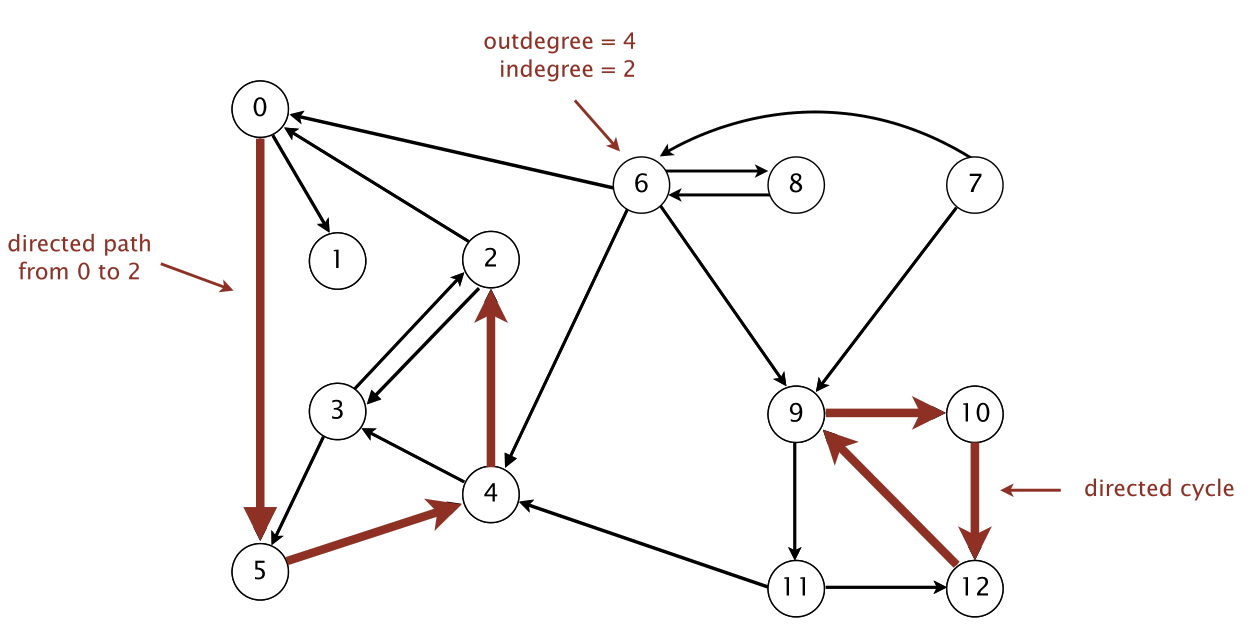
\includegraphics[width=\textwidth]{img/digrafo.png}
    \caption{Fonte: \cite{sedgewick2014algorithms}}
  \end{figure}

\end{frame}

\begin{frame}
  \frametitle{Arestas valoradas}

  Um outra variação da modelagem de grafos é quando as arestas possuem \tcb{valores} (ou pesos).

  \begin{figure}[h]
    \centering
    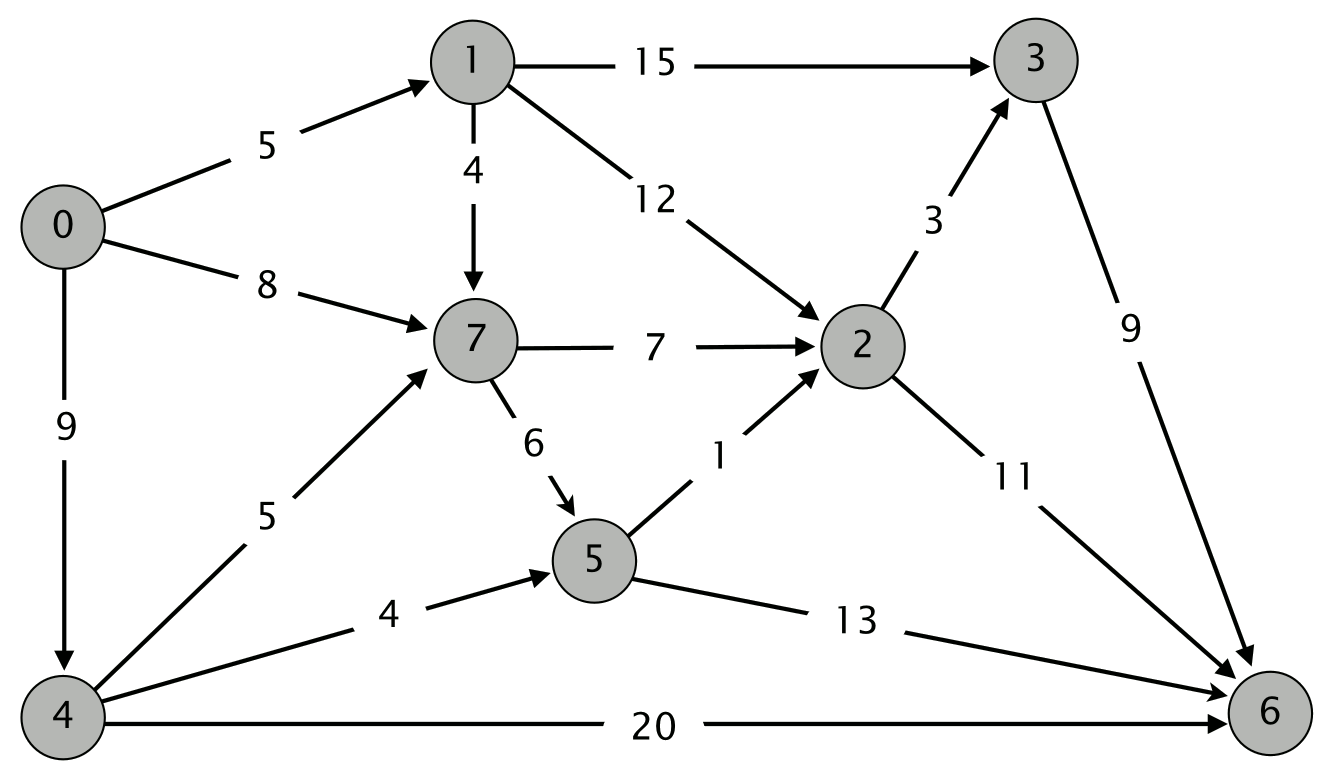
\includegraphics[width=.7\textwidth]{img/peso.png}
    \caption{Fonte: \cite{sedgewick2014algorithms}}
  \end{figure}

  Pesos nas arestas permitem a modelagem de um conjunto maior de problemas.

\end{frame}

\begin{frame}
  \frametitle{Arestas valoradas}

  É importante notar que tanto grafos \textbf{não direcionados} quanto \textbf{direcionados} podem ter arestas com pesos.

  \begin{figure}[h]
    \centering
    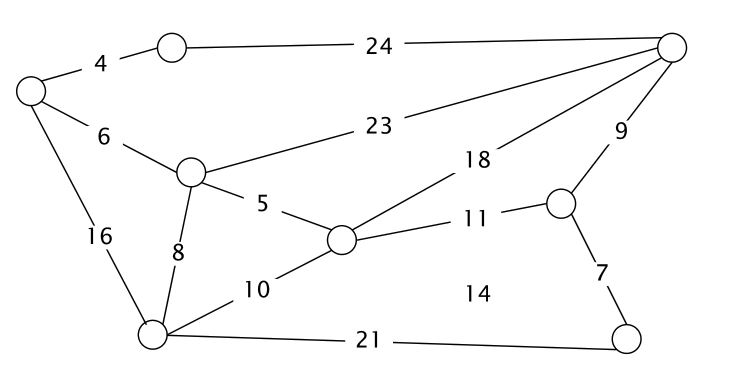
\includegraphics[width=\textwidth]{img/peso_nao_direcionado.png}
    \caption{Fonte: \cite{sedgewick2014algorithms}}
  \end{figure}

\end{frame}

\section{Implementação}

\begin{frame}[fragile]
  \frametitle{Estrutura para Listas de Adjacências de\\Grafos Direcionados com arestas valoradas}

\begin{minted}[frame=lines,framesep=2mm,baselinestretch=1,fontsize=\small,linenos]{c}
struct node {
  int to;               // destination node of edge
  link next;           // next element in adjacency list
  double wt;           // cost of edge
};
typedef struct node *link;

struct digraph {
  int V;               // number of vertices
  int E;               // number of edges
  link *adj;           // adjacency list
};

typedef struct graph *Graph;
typedef struct { int from; int to; } Edge;
\end{minted}

\end{frame}

\begin{frame}[fragile]
  \frametitle{Criação de um Grafo}

\begin{minted}[frame=lines,framesep=2mm,baselinestretch=1,fontsize=\normalsize,linenos]{c}
Digraph DIGRAPHinit(int V) {
  int v;
  Digraph G = malloc(sizeof *G);
  G->V = V; G->E = 0;
  G->adj     = malloc(V * sizeof(*G->adj));
  if (G->adj == NULL){
     fprintf(stderr, "Out of memory in GRAPHinit()\n");
     exit(EXIT_FAILURE);
  }

  for (v = 0; v < V; v++) G->adj[v]  = NULL;

  return G;
}
\end{minted}
\end{frame}

\begin{frame}[fragile]
  \frametitle{Inserção de Aresta}

\begin{minted}[frame=lines,framesep=2mm,baselinestretch=1,fontsize=\normalsize,linenos]{c}
void DIGRAPHinsertE(Digraph G, Edge e, double d) {
  int v = e.from;
  int w = e.to;
  G->adj[v] = NEW(w, G->adj[v], d);
  G->E++;
}
\end{minted}

\end{frame}

\section{Busca em Profundidade e em Largura}

\begin{frame}[c]
  \frametitle{Funcionamento em Grafos Direcionados}

  
  Os algoritmos de Busca em Profundidade e em Largura utilizados em Grafos Não Direcionados
  também podem ser utilizados em Grafos Direcionados.
\end{frame}

\begin{frame}[c]
  \frametitle{Detalhe Busca em Largura}

  Um detalhe importante é que, em grafos com arestas valoradas, a busca em largura pode \textbf{não} entregar
  o menor caminho correto (considera apenas o número de arestas e não o peso).

  Para o cálculo de menor caminho em grafos direcionados e com arestas valoradas, temos outros algoritmos.
\end{frame}

\section{Menor Caminho}

\begin{frame}
  \frametitle{Algoritmo de Dijkstra}

  Para grafos direcionados com arestas valoradas (sem pesos negativos) podemos utilizar o Algoritmo de Dijkstra.
  
  \begin{figure}[h]
    \centering
    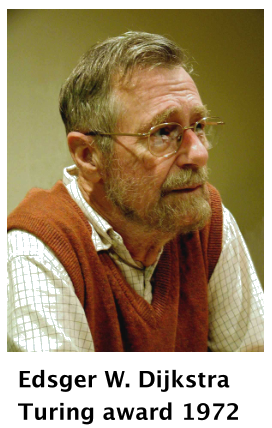
\includegraphics[width=.3\textwidth]{img/dijkstra.png}
    \caption{Fonte: \cite{sedgewick2014algorithms}}
  \end{figure}
  
  O Algoritmo de Dijkstra encontra o menor caminho entre um vértice inicial e todos os outros alcançáveis por ele.

\end{frame}

\begin{frame}
  \frametitle{Relaxação de Aresta}

  O Algoritmo de Dijkstra se baseia no conceito de \tcb{relaxação de aresta}:\\

  \tcb{Relaxação da aresta $e = v \rightarrow w$}
  \begin{itemize}
    \item \texttt{distTo[v]}: é o comprimento do menor caminho \tcr{conhecido} de $s$ até $v$;
    \item \texttt{distTo[w]}: é o comprimento do menor caminho \tcr{conhecido} de $s$ até $w$;
    \item \texttt{edgeTo[w]}: é a última aresta no menor caminho \tcr{conhecido} de $s$ até $w$;
    \item Se $e = v \rightarrow w$ entrega um menor caminho para $w$ através de $v$ então atualiza \texttt{distTo[w]} e \texttt{edgeTo[w]}.
  \end{itemize}

\end{frame}

\begin{frame}
  \frametitle{Relaxação de Aresta}
  
  \begin{figure}[h]
    \centering
    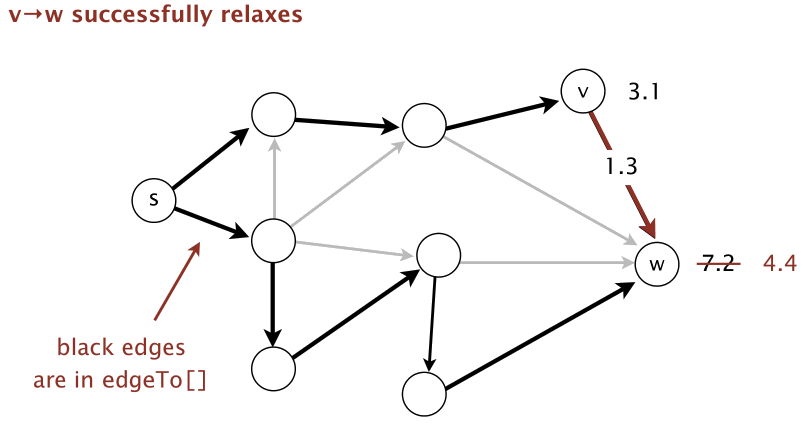
\includegraphics[width=\textwidth]{img/relaxacao.png}
    \caption{Fonte: \cite{sedgewick2014algorithms}}
  \end{figure}
\end{frame}

\begin{frame}
  \frametitle{Algoritmo de Dijkstra}
  O Algoritmo tem os seguintes passos:

  \begin{enumerate}
    \item Escolher o vértice $v$ não visitado com menor distância a partir de $s$ até o momento;
    \item Marcar vértice como visitado;
    \item Realizar a relaxação de todas as arestas que tem origem no vértice $v$.
  \end{enumerate}
\end{frame}

\begin{frame}
  \frametitle{Exemplo Algoritmo de Dijkstra}
  
  \multiinclude[<+->][format=png, graphics={width=\textwidth}]{img/dijkstra/dijkstra}
\end{frame}

\begin{frame}
  \frametitle{Referências utilizadas na apresentação}
  \bibliography{referencias}
\end{frame}
% ==========================================

\end{document}
